\documentclass[a4paper,11pt]{article}
\usepackage{a4wide}
\usepackage[english]{babel}
\usepackage{graphicx}
\usepackage{floatflt}


\begin{document}

\title{Example model:\\Available primitives for development of OpenFLUID functions}
\maketitle


This example is based on a flux model involving 3 simulation functions, 
applied to a spatial domain composed of 13 units distributed into 2 unit classes. 
It aims at showing how values of variables are produced and used in a spatially distributed way.

\bigskip
\bigskip

\section{Overview}

\subsection{Flux model}

\begin{floatingfigure}[r]{6cm}
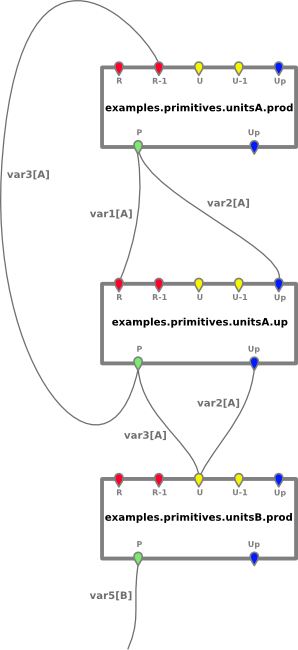
\includegraphics[width=5cm]{openfluid-engine_example-primitives_en/model.png}
\end{floatingfigure}
The flux model is composed of 3 simulations functions :\\
\begin{itemize}
\item examples.primitives.unitsA.prod
\item examples.primitives.unitsA.up
\item examples.primitives.unitsB.prod
\end{itemize}
The examples.primitives.unitsA.prod function produces values for 
variable var1 and var2 on units of class A, and requires values for var3 on units of class A 
on a previous time step.\\
The examples.primitives.unitsA.up function produces values for variable var3 on units of class A, 
updates values for variable var2 on units of class A, and requires values for var1 on units of class A.\\
The examples.primitives.unitsB.prod function produces values for variable var5 on units of class B,
and requires values for var2 and var3 on units of class A.\\
The flux model is defined in the model.xml file.

\bigskip
\bigskip

\subsection{Spatial domain}

The spatial domain is composed of 13 units, distributed into 2 unit classes 
(class A and class B). The connections between 
units are defined for each unit independently, as "to" units. The process order 
depends on these connections. This spatial domain is represented as a graph, 
where nodes are units and edges are connections between units.\\
The spatial domain is defined in *.ddef.xml file(s). 

\begin{center}
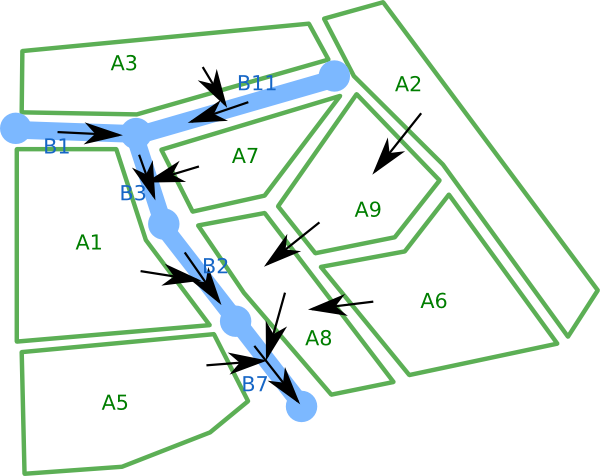
\includegraphics[width=8cm]{openfluid-engine_example-primitives_en/domain.png}
\end{center}


\bigskip
\bigskip

\subsection{Simulation}

The simulation will run from January 1st, 2001, at 00:00:00 to January 15th, 2001, at 08:01:02.
The fixed time step is 3600 seconds (1 hour).\\
\noindent The run configuration is defined in the run.xml file.\\

\noindent All variables of all unit classes (A and B) are saved in files. The output
configuration is defined in the output.xml file.

\bigskip
\bigskip

\section{Run this example}

In order to run this example, the following programs and libraries are required:
\begin{itemize}
\item CMake build system
\item GCC compiler
\item Boost libraries
\item OpenFLUID-engine
\end{itemize}

\noindent All required operations will be executed through a command line terminal,
and will be completed through 3 steps: configuration, build and run.

\subsection{Configure}

The configuration step will configure the build according to the used platform. 
First of all, the config.in.cmake file for each simulation function should be 
adapted, in order to install the resulting built functions in a place where the 
openfluid engine program can reach them.\\

\noindent The configuration of the build can be performed using one of the two
following ways :
\begin{itemize}
\item in-source build : the build files will be mixed with the source files 
\item out-of-source build : the build files will be separated from the source files,
and placed into a choosen directory
\end{itemize}
 

\noindent For configuring an in-source build:\\
1) run command \texttt{cmake .}\\

\noindent For configuring an out-of-source build:\\
1) make a subdirectory for build results (\texttt{\_build} for example)\\
2) change current directory to this subdirectory\\
3) run command \texttt{cmake ..}\\
4) run command \texttt{make install}\\

\subsection{Build}

If the configuration step has passed, the command to launch the build is
\texttt{make} when the GNU Make tools are used, or the corresponding command
if another build system is used.\\
If the installation destination has been configured, the \texttt{make install}
command should be run (or the corresponding command).   


\subsection{Run}

In order to run a simulation using these example functions, the command to run is:\\
\texttt{openfluid-engine -i /path/to/inputdata -o /path/to/outpudir}.\\

\noindent In case of the example simulation functions are not installed in a standard path 
searched by openfluid-engine, the \texttt{-p} command line option should be used 
to add specific search paths. 


\end{document}